% time values for run8 and run9
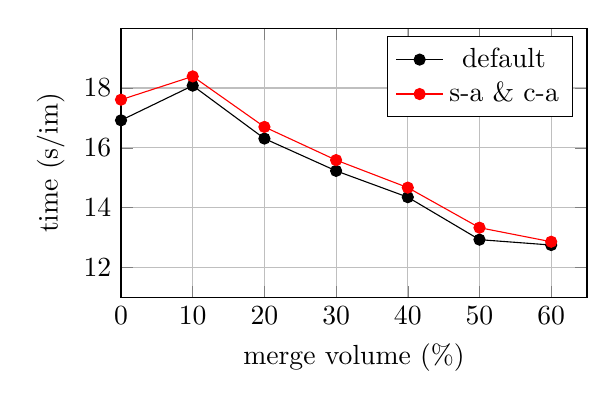
\begin{tikzpicture}
\begin{axis}[
    title={},
    height=5cm,
    width=7.5cm,
    xlabel={merge volume (\%)},
    ylabel={time (s/im)},
    xmin=0, xmax=65,
    ymin=11, ymax=20,
    xtick={0,10,20,30,40,50,60},
    ytick={12,14,16,18},
    legend pos=north east,
    xmajorgrids=true,
    ymajorgrids=true,
]

\addplot[
    color=black,
    mark=*
    ]
    coordinates {
    (0,16.92)(10,18.08)(20,16.31)(30,15.23)(40,14.35)(50,12.93)(60,12.75)
    };
    
\addplot[
    color=red,
    mark=*
    ]
    coordinates {
    (0,17.61)(10,18.39)(20,16.70)(30,15.59)(40,14.67)(50,13.33)(60,12.86)
    };
    
\legend{default, s-a \& c-a}
    
\end{axis}
\end{tikzpicture}